\documentclass{msuposter}

\usepackage{lipsum}
\usepackage{multirow}
\usepackage{tikz,wrapfig}
\newcommand{\mR}{\mathbb{R}}
\newcommand{\mN}{\mathbb{N}}
\newcommand{\cT}{\mathcal{T}}
\newcommand{\uh}{u_h}
\newcommand{\qh}{q_h}
\newcommand{\ph}{p_h}
\newcommand{\qhat}{\hat{q}}
\newcommand{\uhat}{\hat{u}}
\newcommand{\cB}{\mathcal{B}}
\newcommand{\cL}{\mathcal{L}}
\newcommand{\cO}{\mathcal{O}}
\newcommand{\euhat}{\hat{e}_{\uh}}
\newcommand{\eqhat}{\hat{e}_{\qh}}
\newcommand{\cP}{\mathcal{P}}
\newcommand{\projh}{\mathcal{S}}
\newcommand{\eu}{e_u}
\newcommand{\ep}{e_p}
\newcommand{\eq}{e_q}
\newcommand{\xiu}{\xi_u}
\newcommand{\xip}{\xi_p}
\newcommand{\xiq}{\xi_q}
\newcommand{\xiuhat}{\hat{\xi}_u}
\newcommand{\xiqhat}{\hat{\xi}_q}
%\theoremstyle{definition}
%\newtheorem{definition}{Definition}[section]
%\newtheorem{example}{Example}[section]
%\theoremstyle{plain}
%\newtheorem{theorem}{Theorem}[section]
%\newtheorem{corollary}{Corollary}[theorem]
%\newtheorem{lemma}[theorem]{Lemma}
%\newtheorem{proposition}[theorem]{Proposition}
\title{Local discontinuous Galerkin methods with novel basis for fractional diffusion equations with non-smooth solutions}
\author{\href{http://lylyu.com/}{\textbf{Liyao Lyu}} $^a$,Zheng Chen$^b$}
\institute{
$^a$Department of Computational Mathematics, Science and Engineering, Michigan State University
\\
$^b$Department of Mathematics, University of Massachusetts
}

\newcommand{\colwidth}{0.3\linewidth}

\begin{document}
\begin{frame}{}
\begin{columns}[t]
\begin{column}{\colwidth}
\begin{block}{Introduction}
Consider the equations in the form
\begin{equation}\label{eqn:problem}
\frac{\partial u(x,t)}{\partial t} = d \frac{\partial^{\beta} u(x,t)}{\partial x^\beta} + f(x,t), \quad x\in[a,b],\quad \beta\in(1,2),\quad  d>0
\end{equation}
The fractional derivative here is a Caputo derivative
\begin{equation}\label{eqn:def_cd}
{}_a^{C}D_{x}^{\alpha} v(x)=\frac{1}{\Gamma(n-\alpha)} \int_{a}^{x}(x-\xi)^{n-\alpha-1} \frac{d^{n} v(\xi)}{\mathrm{d} \xi^{n}} \mathrm{d} \xi, \quad x>a, \quad \alpha \in[n-1, n)
\end{equation}
The equation \eqref{eqn:problem} can be rewritten into the following system
\begin{equation}\label{local DG}
\begin{aligned}
&\frac{\partial u(x,t)}{\partial t} - \sqrt{d} \frac{\partial q(x,t)}{\partial x} = f(x,t) & \text{in }\Omega_T,\\
& q-_{a}D_{x}^{\beta-2} p(x,t) =0 & \text{in }\Omega_T,\\
& p- \sqrt{d}\frac{\partial u(x,t)}{\partial x}=0& \text{in }\Omega_T,
\end{aligned}
\end{equation}
Local discontinuous Galerkin methods were developed for fractional diffusion equations,
and demonstrated to achieve optimal order of accuracy both theoretically and computationally for smooth enough underlying solutions.
\textbf{However, the order degeneracy is observed when applied to problems with non-smooth solutions.} Consider solving a non-smooth problem with a solution $u(\cdot\, ,t)\in H^\alpha$, the LDG method using finite element space $V^k$ of piecewise polynomials with degree up to $k$, will achieve an error with a theoretical order $\min\{k+1,\alpha\}$, and the numerical order is observed to be like $\min\{k+1,\alpha+0.5\}$

\end{block}
\begin{block}{Novel approximation space and mesh}
	Consider that the solution to problem \eqref{eqn:problem} has an weak singularity at the left end of the domain, and is of form 
	\begin{equation}
	\label{func:solution form}
	w(x) (x-a)^\beta
	\end{equation} 
	with some unknown but smooth function $w(x)$.
	\\
	Near the end $x=a$, we adopt the mapped polynomial functions $P^k((x-a)^\gamma)$ as basis functions to approximate the solution, with $\frac{1}{\gamma}$ being the smallest positive integer makes $\frac{\beta}{\gamma} \in \mathbb{N}$.  
	Since $\beta \in (1,2)$, it is clear that $\gamma \in (0,1)$.\\
	
	We now define the  finite element space $V^k_{\gamma}$for both trial functions and test functions: 
\begin{equation}\label{eqn:functional basis}
V^k_{\gamma} = \left\{v: v\bigr\rvert_{I_j} \in P^k((x-a)^{\gamma}), \text{ if } x_j \leq \hat{x};  \, v \bigr\rvert_{I_j}\in P^{k}(x), \text{ otherwise} \right\}.
\end{equation}
In the domain near starting point the exact solution, being considered as a function of the mapped variable $y = (x-a)^{\gamma}$, is a regular function.
In order to deal with ill-conditioned mass matrix, we adopted graded mesh for the cells with irregular mesh.
\begin{equation}\label{grid:part1}
\begin{aligned}
x_j &= a + \left(\frac{b-a}{N} j \right)^{{1/\gamma}};
\end{aligned}
\end{equation}
for $n < j \leq M$,
\begin{equation}\label{grid:part2}
x_j = b - (M-j)\frac{b-a}{N}.s
\end{equation}
\end{block}
\begin{block}{Semi-defined LDG scheme} 
The semi-discrete LDG scheme to solve systemx is defined as follows. 
Find $\uh, \qh, \ph \in V^k_\gamma$ such that, for all test functions $v, w, z \in V^k_\gamma$ and all $j=1,2,\dots,M$, we have
\begin{equation}\label{eqn:Numerical Scheme}
\begin{aligned}
\left(\frac{\partial \uh(x,t)}{\partial t},\,v(x) \right)_{I_j} +\sqrt{d}\left(\qh(x,t),\,\frac{\partial v(x)}{\partial x}\right)_{I_j} - \sqrt{d}\qhat(x,t) v(x)\Bigr\rvert_{x_{j-1}^+}^{x_j^-}&=(f(x,t),\,v(x))_{I_j},\\
\left( \qh(x,t),\,w(x)\right)_{I_j} - (_{a}D_x^{\beta-2}\ph(x,t),\,w(x))_{I_j}&=0, \\
\left(\ph(x,t),\,z(x)\right)_{I_j} +\sqrt{d}\left(\uh(x,t),\,\frac{\partial z(x)}{\partial x}\right)_{I_j} -\sqrt{d} \uhat(x,t)z(x)\Bigr\rvert_{x_{j-1}^+}^{x_j^-}&=0,
\end{aligned}
\end{equation}
\end{block}
\end{column}



\begin{column}{\colwidth}
\begin{block}{Alternating fluxes}
Here, we use the so-called ``alternating fluxes", which is a popular and attractive choice and defined as
\begin{equation}\label{eqn:Numerical Flux1 inner}
\begin{aligned}
\qhat(x_j,t)&=\qh^+(x_j,t), & \uhat(x_j,t)&=\uh^-(x_j,t); \\
\end{aligned}
\end{equation}
or
\begin{equation}\label{eqn:Numerical Flux2 inner}
\begin{aligned}
\qhat(x_j,t)&=\qh^-(x_j,t), & \uhat(x_j,t)&=\uh^+(x_j,t) \\
\end{aligned}
\end{equation}
at any interior cell interfaces; 
at the domain boundaries, 
\begin{equation}\label{eqn:Numerical Flux \uh BC}
\begin{aligned}
\uhat(a,t)&=0, & \uhat(b,t)&=g(t),  \\
\end{aligned}
\end{equation}
and
\begin{equation}\label{eqn:Numerical Flux \qh BC}
\begin{aligned}
\qhat(a,t)&=\qh^+(a,t), & \qhat(b,t)&=\qh^-(b,t), \\
\end{aligned}
\end{equation}
which reflect the Dirichlet boundary conditions. 
\end{block}

\begin{theorem}[$L^2$ stability]
	The scheme \eqref{eqn:Numerical Scheme} is $L^2$ stable, and the solutions satisfies, for all $t\in [0,T]$, 
	
	\begin{equation}\label{eqn:Stability theorem}
	\begin{aligned}
	\|e_{\uh}(\cdot,t)\|_{L^2}^2 
	+  2\cos ((\beta/2-1)\pi)\int_{0}^{t} \, \|_{a}D_{x}^{\beta/2-1}e_{\ph}(\cdot,t)\|_{L^2}^2 \, dt
	= \|e_{\uh}(\cdot,0)\|_{L^2}^2. 
	\end{aligned}
	\end{equation}
\end{theorem}
	
\begin{theorem}[Error Estimation]\label{thm:accuracy}
	The error for the scheme \eqref{eqn:Numerical Scheme} with flux \eqref{eqn:Numerical Flux1 inner} or \eqref{eqn:Numerical Flux2 inner} and \eqref{eqn:Numerical Flux \uh BC}-\eqref{eqn:Numerical Flux \qh BC} satisfies
	\begin{equation}\label{eqn:accuracy thm}
	\| u - \uh \|_{L^2}  \leq Ch^{k+1}.
	\end{equation}
\end{theorem}

\begin{exampleblock}{$\gamma = 0.5$}
	Consider equation 
	\begin{equation}\label{eqn:exm1}
	\begin{aligned}
	\frac{\partial u(x,t)}{\partial t} = \frac{2 }{3\Gamma(1.5)} \frac{\partial ^{1.5} u(x,t)}{\partial x^{1.5}} - e^{-t} (x^{1.5} +1),\quad x \in (0,1),
	\end{aligned}
	\end{equation}
 on the computational domain $x\in \Omega =(0,1)$. 
	Given initial condition
	\begin{equation}\label{eqn:initial condition for exm1}
	u_0(x) = x^{1.5},
	\end{equation}
	and Dirichlet boundary conditions
	\begin{equation}\label{eqn:boundary condition for exm}
	u(0,t)= 0, \quad u(1,t) =e^{-t}, 
	\end{equation}
	the exact solution is $u(x,t) = e^{-t}x^{1.5}$. 
	\begin{table}
		\centering
		\caption{The error and order of convergence with space $V^1$ on uniform mesh and $V^1_{1/2}$ at $T= 1$.}
		\label{tbl:result k1 beta0.5}
		\begin{tabular}{|c||ll||c||ll|}
			\hline
			\multirow{2}*{$h$}  & \multicolumn{2}{|c|}{$V^1$}  & \multirow{2}*{$h$} & \multicolumn{2}{|c|}{$V^1_{1/2}$ }   \\
			\cline{2-3}
			\cline{5-6}
			~ & error & order & ~ & error & order\\
			\hline
			1/8 & 7.13e-04 & &1/4& 2.41e-03 &\\
			1/16 & 1.82e-04&1.97 & 1/8 &6.17e-04 &1.96 \\
			1/32 & 4.70e-05&1.95 & 1/16 &1.41e-04 &2.12  \\
			1/64 & 1.23e-05&1.92 & 1/32 & 3.46e-05 & 2.03\\
			1/128&3.23e-06& 1.93 & 1/64 & 8.73e-06 & 1.98\\
			\hline
		\end{tabular}
	\end{table}
	
	\begin{table}
		\centering
		\caption{The error and order of convergence for LDG methods with space $V^2$ on uniform mesh and $V^2_{1/2}$ at $T= 1$.}
		\label{tbl:result k2 beta0.5}
		\begin{tabular}{|c||ll||c||ll|}
			\hline
			\multirow{2}*{$h$}  & \multicolumn{2}{|c|}{$V^2$ } & \multirow{2}*{$h$} & \multicolumn{2}{|c|}{$V^2_{1/2}$}   \\
			\cline{2-3}
			\cline{5-6}
			~ & error & order & ~ & error & order\\
			\hline
			1/8 & 6.27e-05 & & 1/4 & 9.85e-05 &\\
			1/16 & 1.48e-05& 2.07 & 1/8 &1.17e-05 &3.06 \\
			1/32 & 3.65e-06&2.02& 1/16 & 1.42e-06 &3.03 \\
			\hline
			\end{tabular}
	\end{table}
	
\end{exampleblock}

\end{column}
\begin{column}{\colwidth}
\begin{exampleblock}{}
\begin{figure}
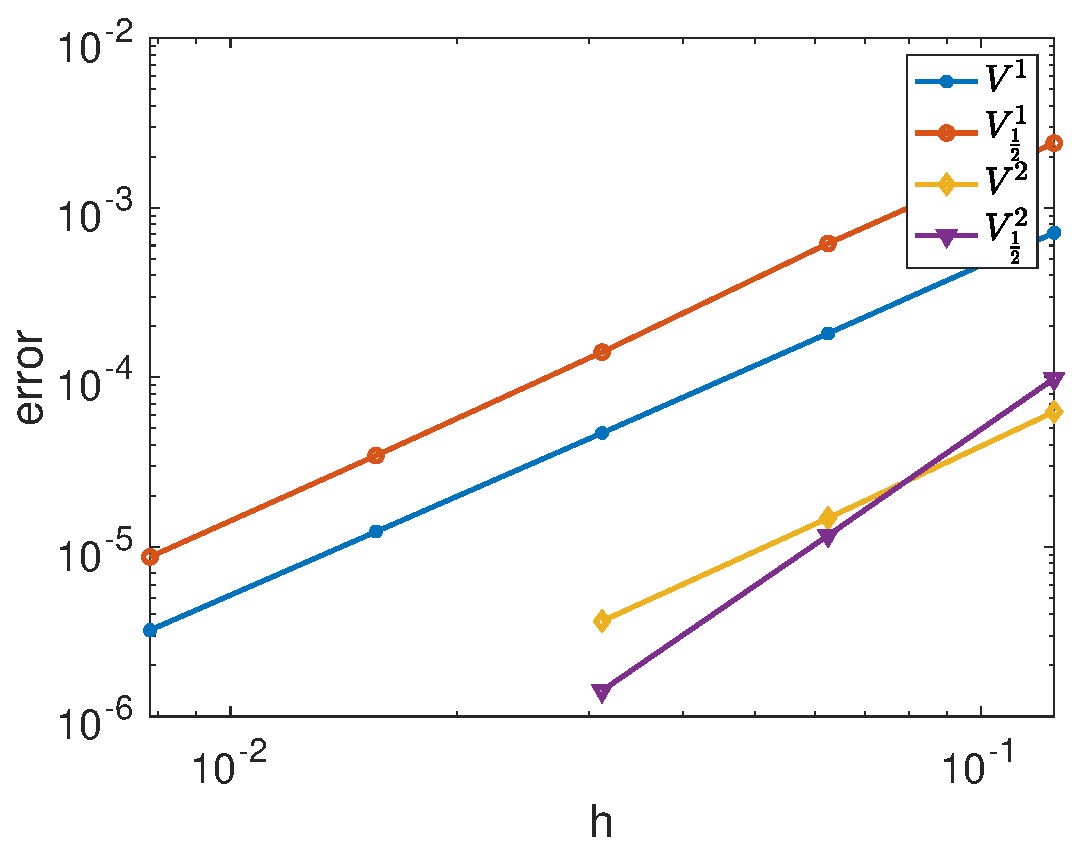
\includegraphics[width=0.5\linewidth]{Figure1}
\end{figure}
\end{exampleblock}

\begin{exampleblock}{$\gamma = 	\frac{1}{3}$}
Consider 
	\begin{equation}
	\begin{aligned}
	\frac{\partial u(x,t)}{\partial t} = \frac{9\sqrt{3}\Gamma(\frac{2}{3}) }{8\pi} \frac{\partial ^{\frac{4}{3}} u(x,t)}{\partial x^{\frac{4}{3}}} - e^{-t} (x^{\frac{4}{3}} +1)
	\end{aligned}
	\end{equation}
	in $\Omega = (0,1)$ with exact solution $u(x)= e^{-t} x^{\frac{4}{3}}$. 
\begin{table}
		\centering
		\caption{The error and order of convergence for LDG methods solving problem with $V^1$ on uniform mesh and $V^1_{1/3}$ on the same mesh as before, {at $T= 0.1$ with cfl $=0.0001$}.}
		\label{tbl:result k1 beta1/3}
		\begin{tabular}{|c|ll||c|ll|}
			\hline
			\multirow{2}*{$h$}  & \multicolumn{2}{|c||}{$V^1$}  & \multirow{2}*{$h$}  & \multicolumn{2}{|c|}{$V^1_{1/3}$}   \\
			\cline{2-3} 
			\cline{5-6}
			~ & error & order & ~ & error & order \\
			\hline
			1/8 & 1.44e-3& & 1/4 & 6.23e-03 & \\
			1/16& 4.14e-4& 1.80 & 1/8 & 1.76e-03 & 1.82 \\
			1/24& 1.98e-4& 1.81& 1/12 & 7.47e-04 & 2.12 \\
			1/32& 1.18e-4& 1.79& 1/16 & 4.22e-04 & 1.98 \\
			1/40& 7.89e-5& 1.81& 1/20 & 2.64e-04 & 2.09 \\
			1/48& 5.65e-5& 1.82& 1/24  & 1.85e-04 & 1.96 \\
			\hline
		\end{tabular}		
	\end{table}
%	
	\begin{table}
		\centering
		\caption{The error and order of convergence for LDG methods solving problem with $V^1$ on uniform mesh and $V^1_{1/3}$ on the same mesh as before, {at $T= 0.1$ with cfl $=0.0001$}.}
		\label{tbl:result k2 beta1/3}
		\begin{tabular}{|c|ll||c|ll|}
			\hline
			\multirow{2}*{$h$}  & \multicolumn{2}{|c||}{$V^2$}  & \multirow{2}*{$h$}  & \multicolumn{2}{|c|}{$V^2_{1/3}$}   \\
			\cline{2-3} 
			\cline{5-6}
			~ & error & order & ~ & error & order \\
			\hline
			1/8 & 2.10e-04 &  &1/4 & 5.19e-04 & \\
			1/16& 5.82e-05 & 1.85  &1/8 & 5.55e-05 & 3.21\\
			1/24& 2.78e-05 & 1.82  &1/12 & 1.58e-05 & 3.07\\
			1/32& 1.65e-05 & 1.81  &1/16 & 7.25e-06 & 2.82\\
			1/40& 1.11e-05 & 1.74  & 1/20 & 2.15e-06 & 2.49\\
			\hline
		\end{tabular}
	\end{table}
	\begin{figure}
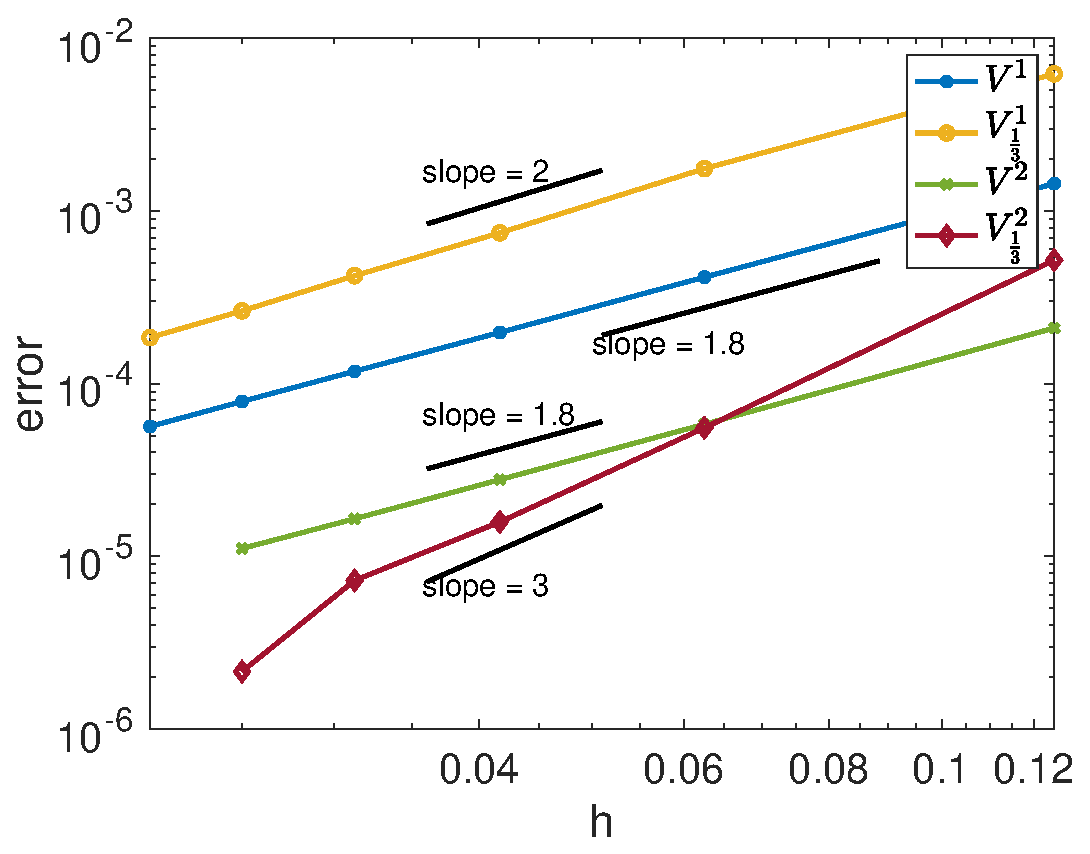
\includegraphics[width=0.5\linewidth]{Figure2}
\end{figure}
\end{exampleblock}
\end{column}
\end{columns}	
\end{frame}
\end{document}
